\documentclass[tikz,border=8pt]{standalone}
\usepackage[T1]{fontenc}
\usepackage[utf8]{inputenc}
\usepackage{tikz}
\usetikzlibrary{arrows.meta,positioning,fit,backgrounds}

\begin{document}
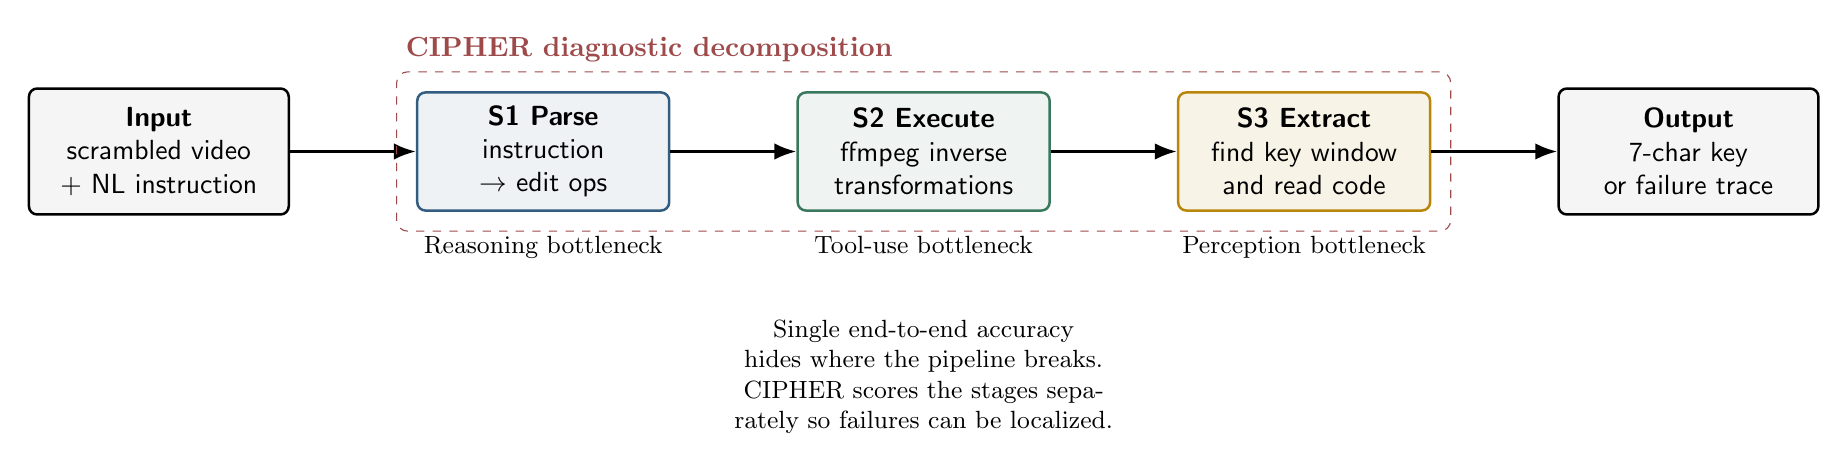
\begin{tikzpicture}[
    font=\sffamily,
    >=Latex,
    stage/.style={
        draw,
        rounded corners=3pt,
        minimum width=3.2cm,
        minimum height=1.5cm,
        align=center,
        line width=0.9pt
    },
    io/.style={
        draw,
        rounded corners=3pt,
        minimum width=3.3cm,
        minimum height=1.6cm,
        align=center,
        fill=gray!8,
        line width=0.9pt
    },
    note/.style={
        font=\small,
        text width=3.2cm,
        align=center
    }
]

\definecolor{cipherblue}{RGB}{50,92,128}
\definecolor{ciphergold}{RGB}{184,134,11}
\definecolor{ciphergreen}{RGB}{58,120,94}
\definecolor{cipherred}{RGB}{158,74,74}

\node[io] (input) at (0,0) {\textbf{Input}\\scrambled video\\+ NL instruction};

\node[stage, draw=cipherblue, fill=cipherblue!8, right=1.6cm of input] (s1) {\textbf{S1 Parse}\\instruction\\$\rightarrow$ edit ops};
\node[note, below=0.18cm of s1] {Reasoning bottleneck};

\node[stage, draw=ciphergreen, fill=ciphergreen!8, right=1.6cm of s1] (s2) {\textbf{S2 Execute}\\ffmpeg inverse\\transformations};
\node[note, below=0.18cm of s2] {Tool-use bottleneck};

\node[stage, draw=ciphergold, fill=ciphergold!10, right=1.6cm of s2] (s3) {\textbf{S3 Extract}\\find key window\\and read code};
\node[note, below=0.18cm of s3] {Perception bottleneck};

\node[io, right=1.6cm of s3] (out) {\textbf{Output}\\7-char key\\or failure trace};

\draw[->, line width=1.1pt] (input) -- (s1);
\draw[->, line width=1.1pt] (s1) -- (s2);
\draw[->, line width=1.1pt] (s2) -- (s3);
\draw[->, line width=1.1pt] (s3) -- (out);

\node[draw=cipherred, dashed, rounded corners=4pt, inner sep=7pt, fit=(s1)(s2)(s3)] (fitbox) {};
\node[anchor=south west, text=cipherred, font=\bfseries] at (fitbox.north west) {CIPHER diagnostic decomposition};

\node[note, below=1.25cm of s2, text width=8.4cm] {
Single end-to-end accuracy hides where the pipeline breaks.\\
CIPHER scores the stages separately so failures can be localized.
};

\end{tikzpicture}
\end{document}
